\chapter{\textsc{AD et DA}}

Les Convertisseurs Analogique-Numérique (ADC pour \textit{Analog to Digital Converter}) et Numérique-Analogique (DAC pour \textit{Digital to Analog Converter}) sont des éléments importants de toute chaîne d'acquisition de donnée.\\
En effet, les opérations complexes de traitement de signal sont aujourd'hui exécutées par des circuits numériques, dont les microcontrôleurs font partie. Pour être traités par un microcontrôleur, les signaux analogiques doivent donc être convertis en nombres.\\
La figure \ref{fig:Acq_Chain} illustre une chaîne typique d'acquisition de donnée.

\begin{figure}[htb]
  \centering
  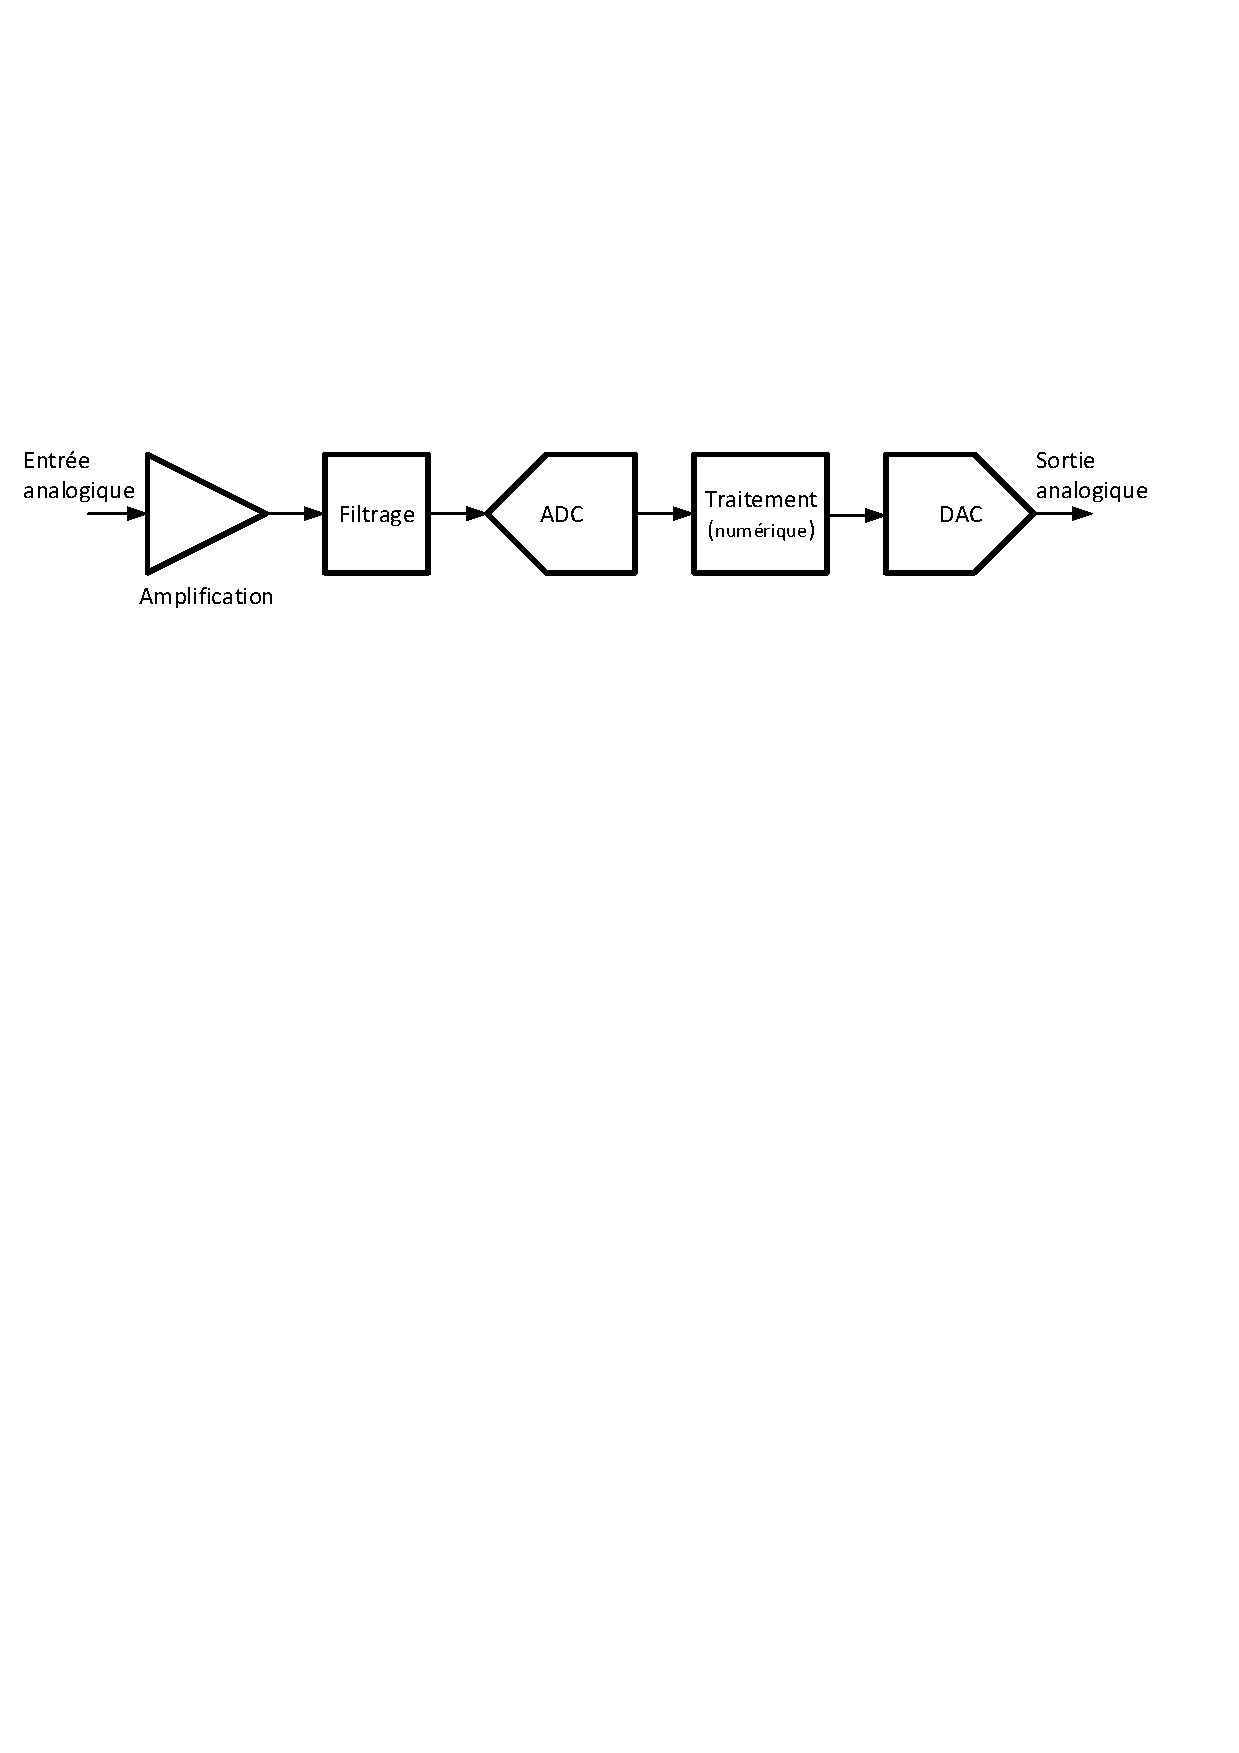
\includegraphics [angle=0, width=14cm]{./Figures/Chap11_ADC/Acq_Chain.pdf}
  \rule{35em}{0.5pt}
  \caption{Chaîne d'acquisition et traitement de signal}
  \label{fig:Acq_Chain}
\end{figure}

\section{Convertisseur AD}
L'ADC est un circuit dont la fonction est de convertir une grandeur physique $V_{in}$ - en général une tension, parfois un courant - en un nombre N représenté sur plusieurs bits, "proportionnel" à cette grandeur physique.
Le terme proportionnel est abusif dans la mesure où la fonction de transfert $N = f(V_{in})$ est une fonction en escalier, comme illustré à la figure \ref{fig:ADC_Fonction}.

\begin{figure}[htb]
  \centering
  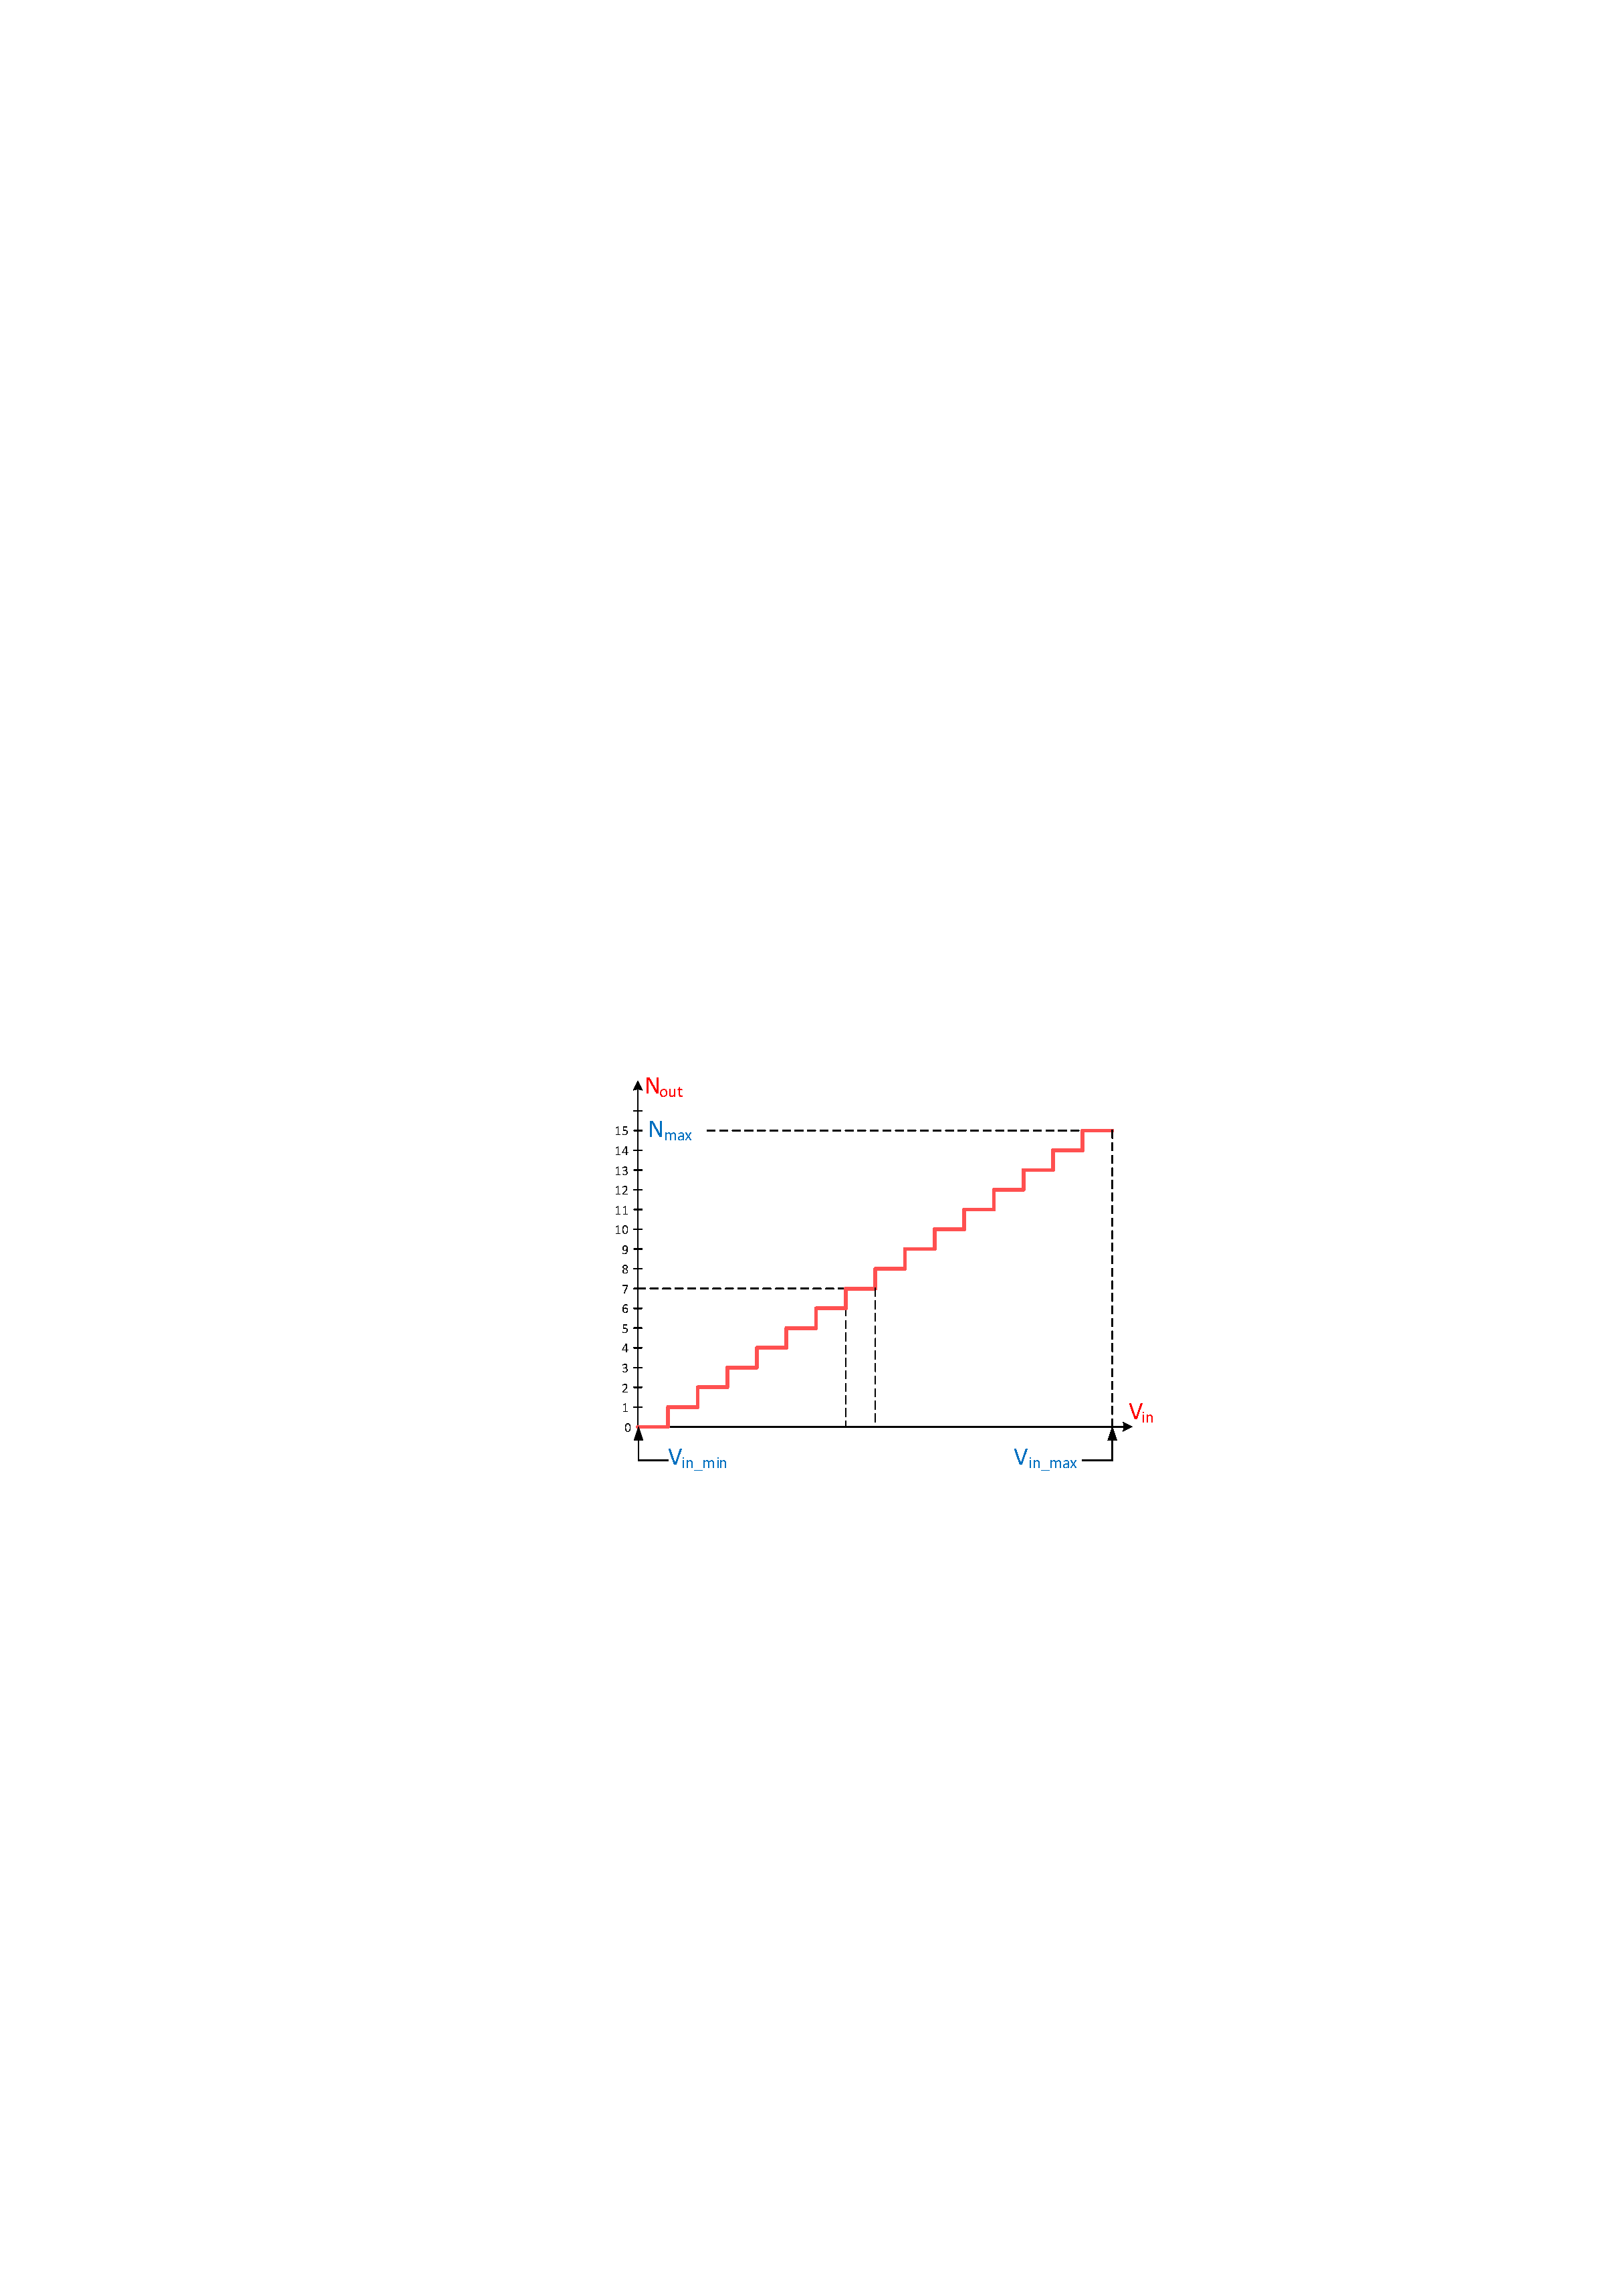
\includegraphics [angle=0, width=10cm]{./Figures/Chap11_ADC/ADC_Fonction.pdf}
  \rule{35em}{0.5pt}
  \caption{Fonction de transfert d'un ADC idéal 4-bits}
  \label{fig:ADC_Fonction}
\end{figure}

Les caractéristiques importantes de cette fonction de transfert sont:
\begin{itemize}[label=\textbullet,font=\small]
  \item l'intervalle des tensions d'entrée $[V_{in\_min}, V_{in\_max}$]
  \item la résolution, égale à $log_{2}(N_{max})$
  \item les imperfections qui l'entachent, et qui sont:
  \begin{itemize}[label=\textbullet,font=\small]
    \item offset
    \item erreur de gain
    \item "non linéarité" de la fonction
  \end{itemize}
\end{itemize}

Il existe plusieurs méthodes pour convertir une grandeur physique en un nombre. Elles se différencient principalement par la résolution atteignable et la rapidité du processus de conversion, et aussi par leur complexité.\\
Dans les microcontrôleurs, le convertisseur AD le plus souvent rencontré est le convertisseur à approximations successives, dont l'avantage est d'offrir un bon compromis entre résolution et rapidité, pour une consommation de courant très faible.

\section{Convertisseur à approximations successives}

Ce type de convertisseur utilise un processus de dichotomie pour traduire progressivement une tension analogique en un nombre. Le temps de conversion est fonction du nombre de bits souhaités.\\
Le principe est illustré à la figure \ref{fig:ADC_SAR_Diagram}.

\begin{figure}[htb]
  \centering
  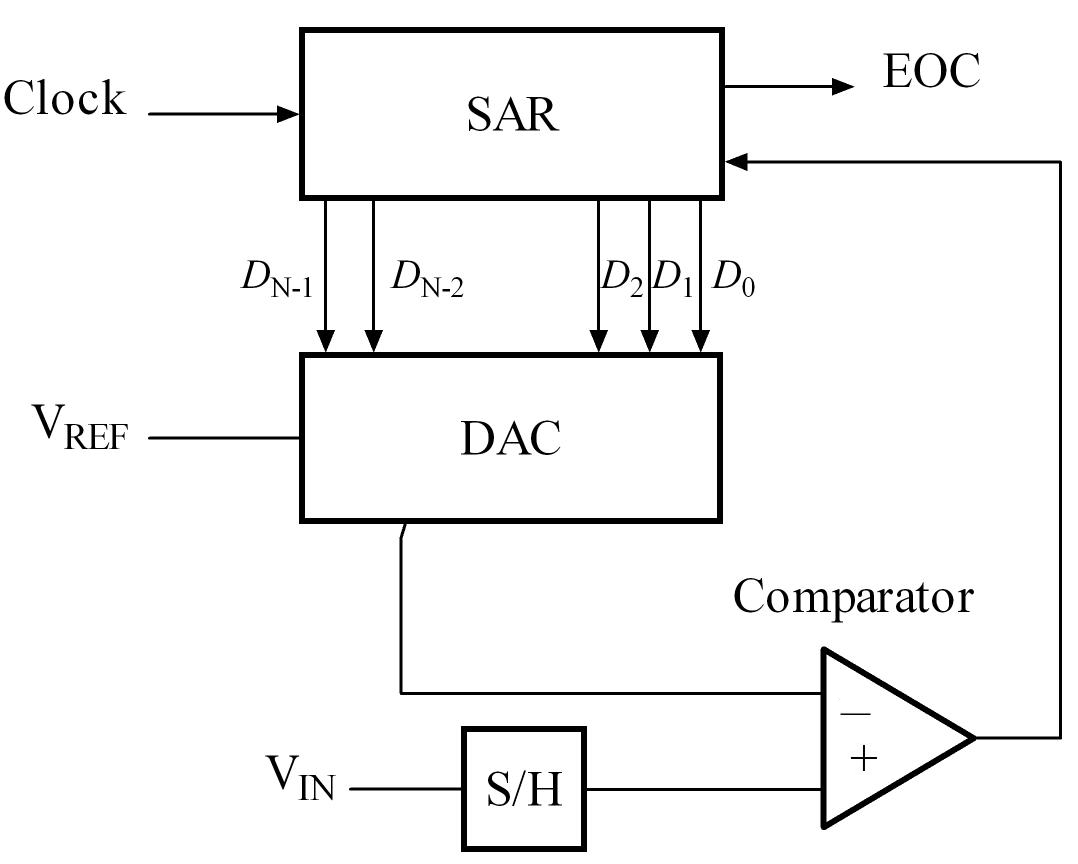
\includegraphics [angle=0, width=10cm]{./Figures/Chap11_ADC/SA_ADC_block_diagram.png}
  \rule{35em}{0.5pt}
  \caption{Principe du convertisseur à approximations successives}
  \label{fig:ADC_SAR_Diagram}
\end{figure}

Un séquenceur (généralement nommé SAR pour \textit{Successive Approximation Register}), couplé à un convertisseur Digital-Analogique (DAC) génère une tension analogique, qui est comparée au signal à convertir.
Le résultat de cette comparaison est alors introduit dans le SAR, qui va le prendre en compte, pour la suite du processus de dichotomie, jusqu'à complétion. La figure \ref{fig:ADC_SAR} illustre la chronologie du processus de conversion, dans le cas d'un ADC 4-bits.\\
Dans cet exemple, le DAC est capable de générer 16 tensions notées $x.FS$ (FS signifie \textit{Full Scale}), avec $0 \leqslant x \leqslant 15$. Les valeurs minimale et maximale de ces tensions sont appelées \textit{tensions de référence}.\\
Le test du MSB détermine si $V_{in}$ est supérieur ou inférieur à $\scriptstyle {}^1\!/\!_2.FS$. Dans l'exemple, dès lors que $V_{in} \leqslant \scriptstyle {}^1\!/\!_2.FS$, le MSB vaut 1. Pour tester le bit de poids inférieur (MSB-1), le séquenceur commande le DAC pour qu'il génère $\scriptstyle {}^3\!/\!_4.FS$. Cette fois,  $V_{in} \geqslant \scriptstyle {}^3\!/\!_4.FS$, donc (MSB-1) = 0; ceci signifie qu'il ne fallait pas ajouter $\scriptstyle {}^1\!/\!_4.FS$ à 
$\scriptstyle {}^1\!/\!_2.FS$ mais $\scriptstyle {}^1\!/\!_8.FS$.\\
Le processus continue ainsi jusqu'à l'obtention du LSB, au rythme d'un bit par étape.

\begin{figure}[htb]
  \centering
  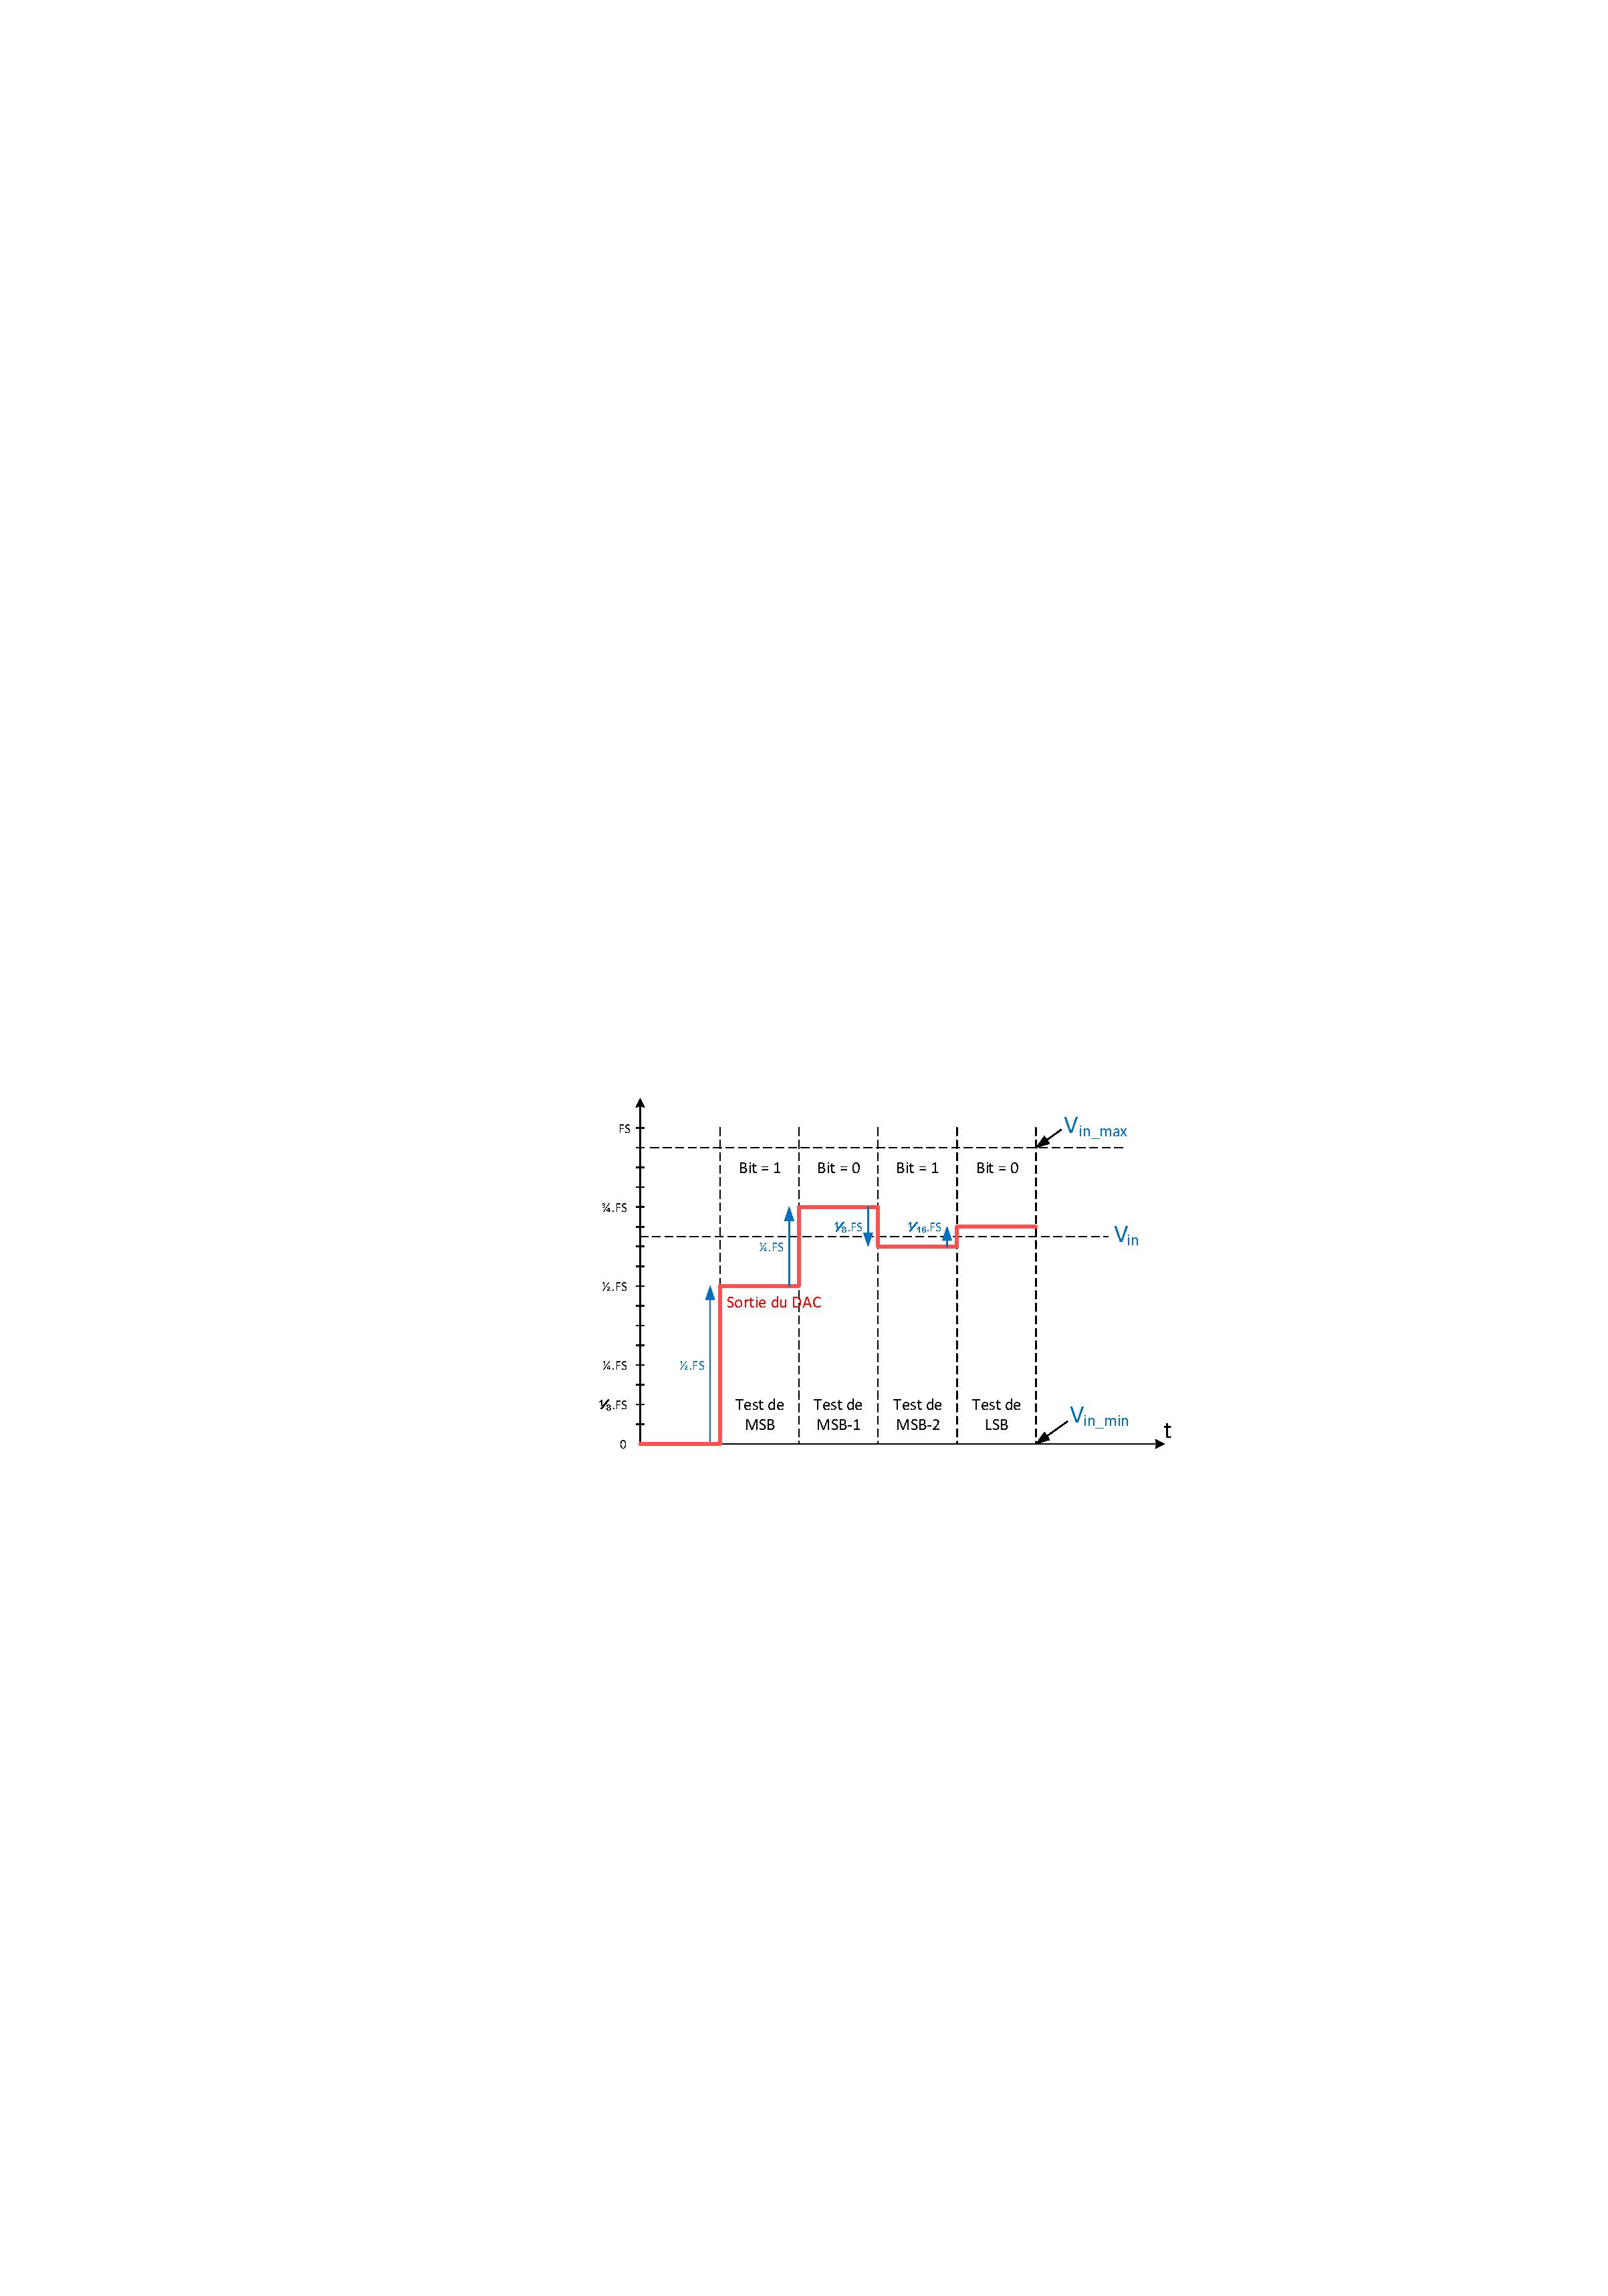
\includegraphics [angle=0, width=13cm]{./Figures/Chap11_ADC/ADC_SAR.pdf}
  \rule{35em}{0.5pt}
  \caption{Etapes de conversion d'un ADC 4-bits à approximations successives}
  \label{fig:ADC_SAR}
\end{figure}

Le convertisseur réalise donc sa conversion en positionnant en premier le bit de poids fort (MSB) et en descendant progressivement jusqu'au LSB.
Ces convertisseurs ont des résolutions d'une douzaine de bits environ, mais peuvent atteindre 16 bits au moyen de technologies spéciales.\\

Il est important de noter que la tension d'entrée doit être mémorisée pendant toute la durée du processus de conversion. Ceci est effectué au moyen d'un circuit auxiliaire appelé "Echantillonneur-Bloqueur" (\textit{Sample and Hold}). Le terme "Echantillonneur" fait référence à l'instant auquel la tension est saisie; "Bloqueur" fait référence à sa mémorisation. 

Le convertisseur DAC peut être construit au moyen de:
\begin{itemize}[label=\textbullet,font=\small]
  \item un diviseur de tension résistif couplé à des interrupteurs
  \item un diviseur de courant de type R-2R
  \item un diviseur de tension à capacités pondérées
\end{itemize}
Le détail de ces circuits sort du cadre de ce cours.

\section{Cas du MSP430}
Les microcontrôleurs MSP430 peuvent contenir plusieurs types de convertisseurs AD:
\begin{itemize}[label=\textbullet,font=\small]
  \item AD 10-bits à approximations successives
  \item AD 12-bits à approximations successives
  \item AD 16-bits Sigma-Delta
\end{itemize}

\subsection{Cas du MSP430F5529}
Ce microcontrôleur contient un convertisseur AD 12 bits à approximations successives avec les caractéristiques suivantes.
\begin{itemize}[label=\textbullet,font=\small]
  \item Plus de 200 kSPS : 200'000 échantillons par seconde
  \item Echantillonneur-Bloqueur avec période programmable, contrôlée par logiciel ou par timers
  \item Lancement des conversions par logiciel ou par timers
  \item Référence de tension interne sélectionnable par logiciel (1.5 V, 2.0 V, ou 2.5 V)
  \item Référence interne ou externe
  \item Jusqu'à 12 canaux d'entrée configurables individuellement
  \item Canaux d'entrée pour capteur de température interne, AVCC, et références externes
  \item Registres de stockage de 16 résultats de conversion
\end{itemize}

\subsection{Schéma de l'ADC 12-bits}
La figure \ref{fig:ADC_Schema} représente le schéma complet du périphérique ADC12, l'ADC 12-bits présent dans le MSP430F5529. 

\begin{figure}[H]
  \centering
  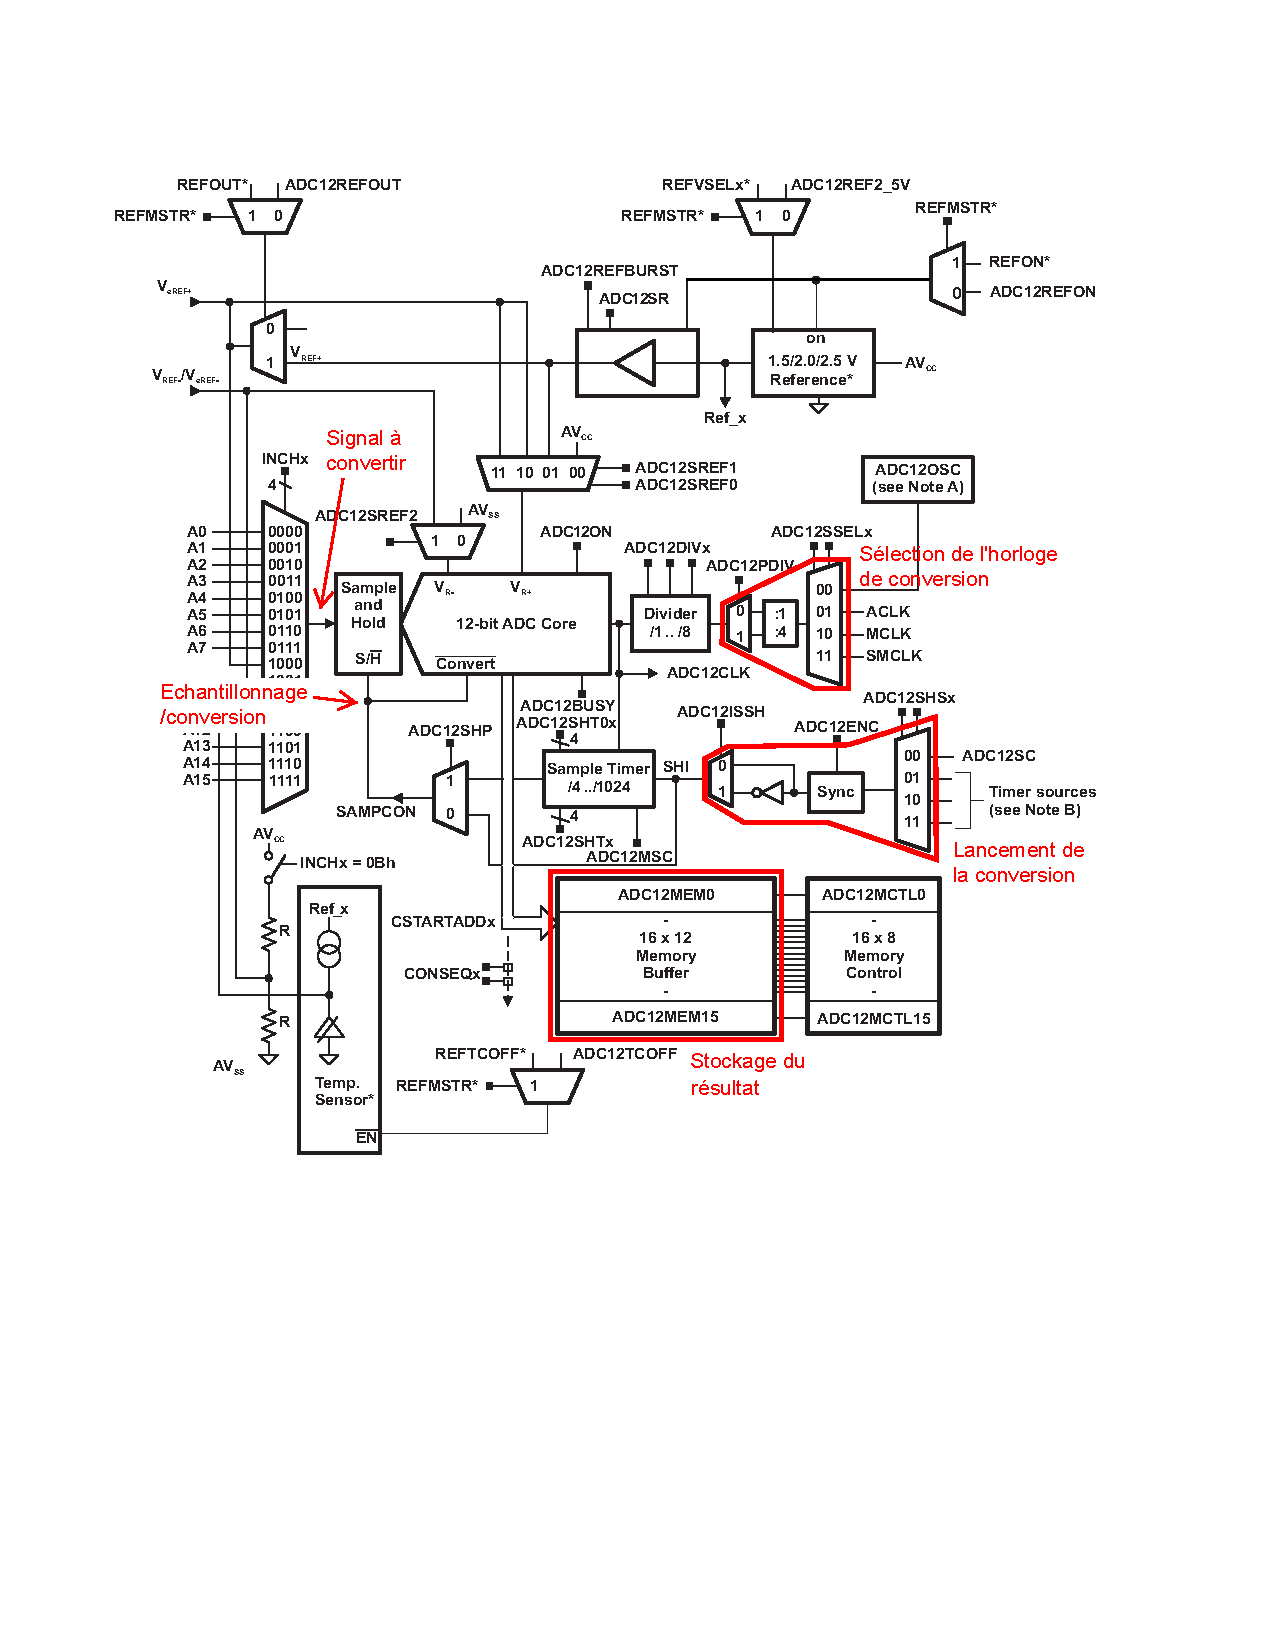
\includegraphics [angle=0, width=16cm]{./Figures/Chap11_ADC/ADC_Schema.pdf}
  \rule{35em}{0.5pt}
  \caption{Schéma du convertisseur ADC12 dans le MSP430F5529}
  \label{fig:ADC_Schema}
\end{figure}

On y trouve:
\begin{itemize}[label=\textbullet,font=\small]
  \item le coeur de l'ADC, avec l'échantillonneur-bloqueur, au centre
  \item le bloc de sélection des références de tension
  \item le bloc de sélection de l'horloge de conversion, qui définit le rythme auquel les bits du résultat sont obtenus
  \item le bloc de lancement d'une conversion. Il est possible de lancer automatiquement des conversions
  \item une mémoire pouvant contenir les résultats de 16 conversions
  \item à gauche, le circuit de sélection du signal à convertir
\end{itemize}

Comme on l'a déjà vu avec d'autres périphériques, les réglages du convertisseur ADC12 se font par le logiciel, en positionnant les champs logiques apparaissant sur le schéma, qui sont accessibles dans des registres de contrôle.

\pagebreak
\subsection{Echantillonnage et conversion}
Le processus de conversion commence par l'échantillonnage du signal d'entrée, puis continue avec la conversion par approximations successives. Le processus est lancé sur le flanc montant du signal SHI, comme indiqué à la figure \ref{fig:ADC12SHP1}.

\begin{figure}[H]
  \centering
  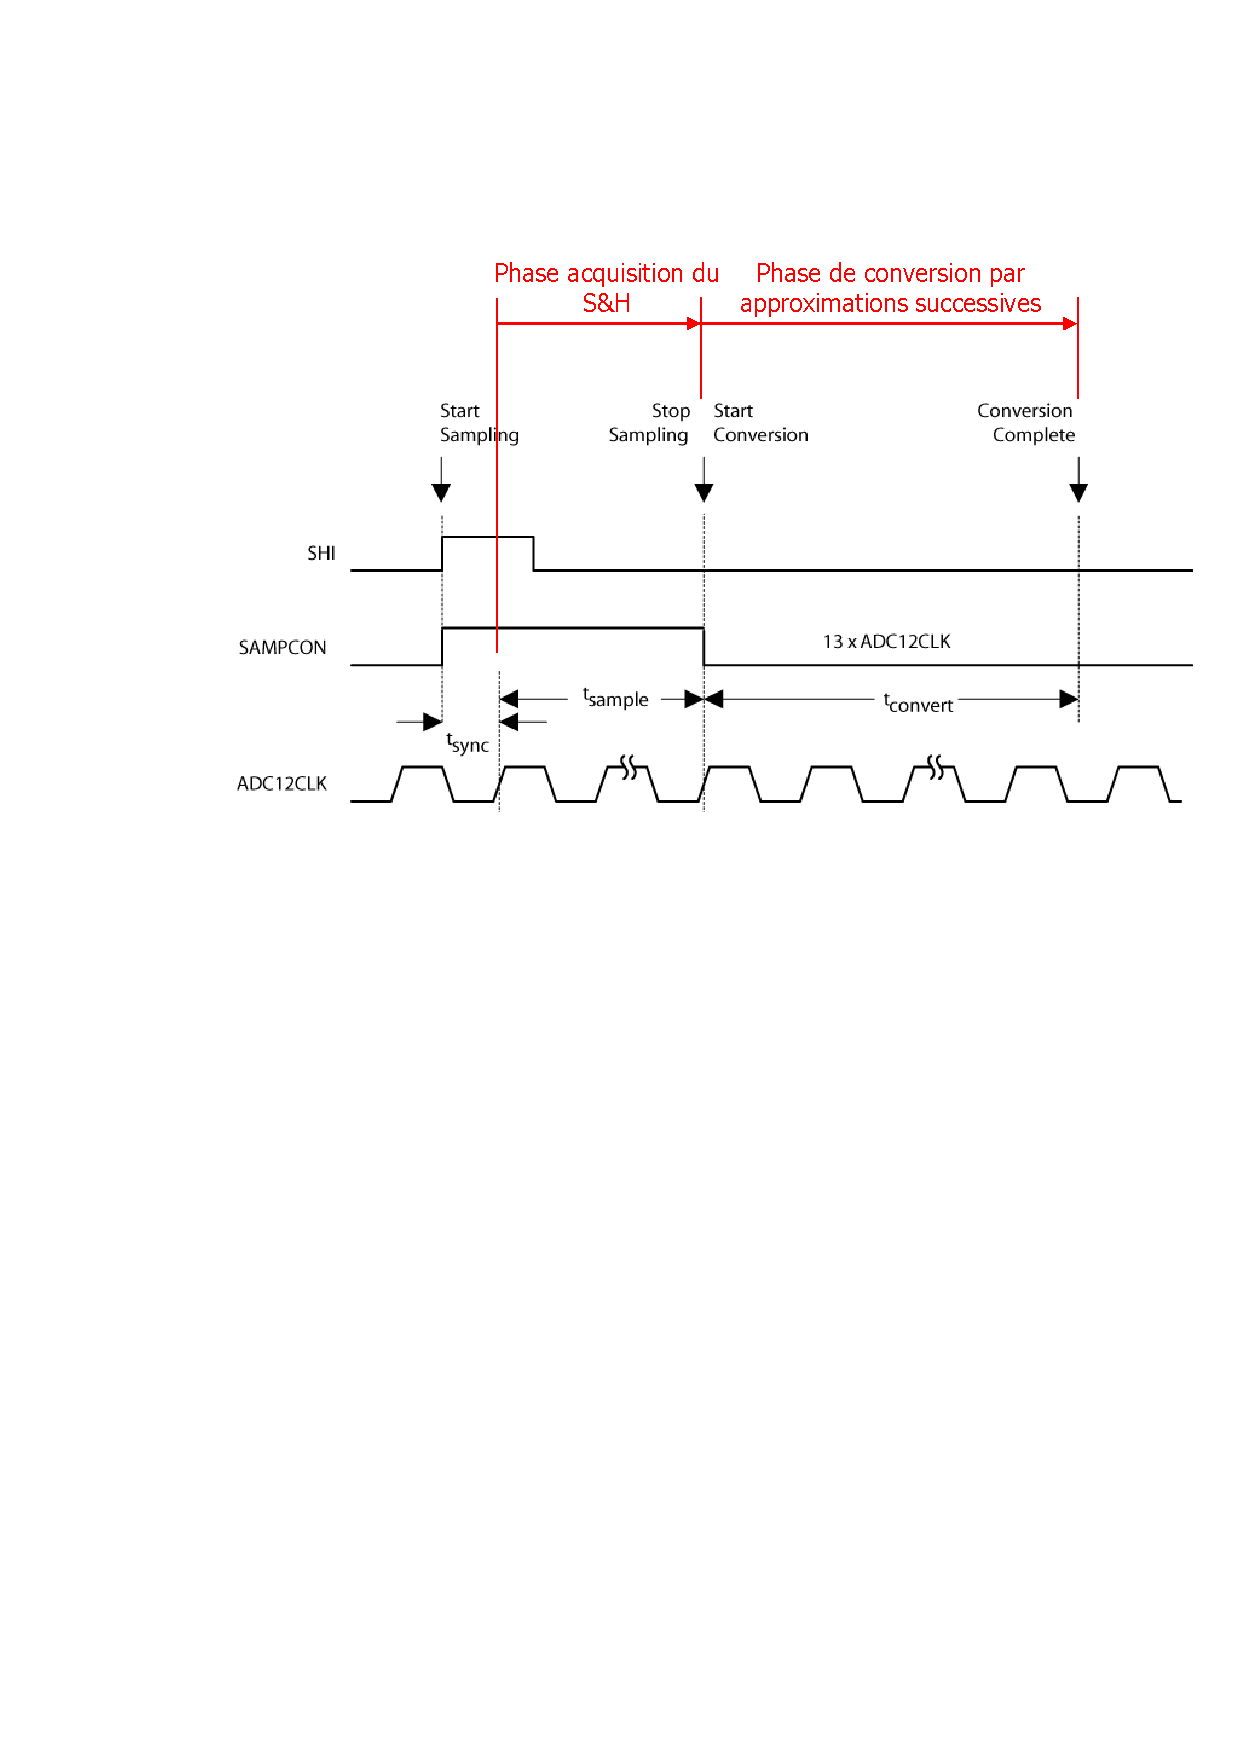
\includegraphics [angle=0, width=14cm]{./Figures/Chap11_ADC/ADC12SHP1.pdf}
  \rule{35em}{0.5pt}
  \caption{Chronogramme du processus d'échantillonnage et conversion (ADC12SHP = 1)}
  \label{fig:ADC12SHP1}
\end{figure}

Le signal SAMPCON (\textit{Sampling Control}) joue un rôle particulier car son flanc montant détermine le début de la saisie du signal d'entrée, qui dure tant que $SAMPCON = 1$. La conversion à proprement parler démarre au flanc descendant de  SAMPCON et dure 13 périodes du signal ADC12CLK pour une conversion sur 12 bits.
La durée du signal SAMPCON doit être réglable pour pouvoir ajuster le temps d'échantillonnage à la résistance interne de la source d'où provient $V_{in}$. En effet, l'entrée de l'échantillonneur-bloqueur (le \textit{Sample and Hold}) est une capacité; sa charge est soumise à une constante de temps qui dépend de la résistance de la source.\\

\subsection{Sélection de l'horloge de conversion}
L'horloge de conversion ADC12CLK rythme le processus de conversion par approximations successives. Elle détermine donc le temps alloué au calcul de chaque bit, du MSB au LSB.\\

Lorsque l'utilisateur souhaite se simplifier la vie (ADC12SHP = 1), elle détermine aussi la durée de l'échantillonnage, via un timer interne à l'ADC\footnote{La durée d'échantillonnage peut aussi être contrôlée par le programme. Dans ce cas (ADC12SHP = 0) le signal SHI contrôle directement la durée d'échantillonnage et la conversion. SHI est alors généré par le programme ou par un des timers à usage général}. Ce timer, noté \textit{Sample Timer}  sur la figure \ref{fig:ADC_Schema} peut générer une durée d'échantillonnage comprise entre 4 et 1024 cycles du signal ADC12CLK.

Les sources d'horloge usuelles (ACLK, SMCLK et MCLK) peuvent être utilisées. Par défaut, un autre signal est disponible, noté ADC12OSC, et dont la fréquence est d'environ 5 MHz.

\subsection{Lancement d'une conversion}
Plusieurs méthodes sont envisageables:
\begin{itemize}[label=\textbullet,font=\small]
  \item lancement par logiciel, en activant le bit ADC12SC (\textit{Start Conversion})
  \item lancement automatique par un timer
\end{itemize}

\subsection{Sélection des références de tension}
Les références de tension déterminent l'intervalle dans lequel la tension à convertir doit se trouver. La borne inférieure peut être égale à GND, mais pas nécessairement. Par contre, la borne supérieure est toujours inférieure à la tension d'alimentation VCC. La raison est que les circuits internes au convertisseur ont besoin d'une marge entre $V_{REF_Sup}$ et VCC pour pouvoir fonctionner correctement.
Le résultat $N_{ADC}$ de la conversion est donné par la formule suivante :

\begin{tabbing}
  \begin{Large}
    \qquad $N_{ADC}=4095.\frac{V_{in}-V_{Ref-}}{V_{Ref+}-V_{Ref-}}$
  \end{Large}
\end{tabbing}


\subsection{Stockage des résultats}
Lorsqu'une conversion est terminée, l'ADC peut émettre une requête d'interruption. Toutefois, dans de nombreuses applications, il est nécessaire de convertir plusieurs tensions différentes. Les raisons peuvent être:
\begin{itemize}[label=\textbullet,font=\small]
  \item les signaux générés par plusieurs capteurs, et connectées sur l'ADC via ses différentes entrées (A0 à A15) doivent être convertis en nombres;
  \item plusieurs valeurs successives d'une même tension doivent être converties, pour pouvoir calculer une moyenne ou y appliquer une fonction de filtrage numérique;
  \item on ne souhaite pas surcharger le CPU avec des interruptions trop fréquentes;
  etc...
\end{itemize}

Pour résoudre ce genre de situation, l'ADC dispose d'une mémoire pouvant contenir jusqu'à 16 résultats de conversion. Il est possible de définir des séquences de conversion, et de faire en sorte qu'une interruption ne soit émise qu'à la fin de la séquence.\\
Chacun des 16 registres de stockage, notés ADC12MEMx est associé à un registre de contrôle noté ADC12MCTLx (x = 0..15).

\begin{figure}[H]
  \centering
  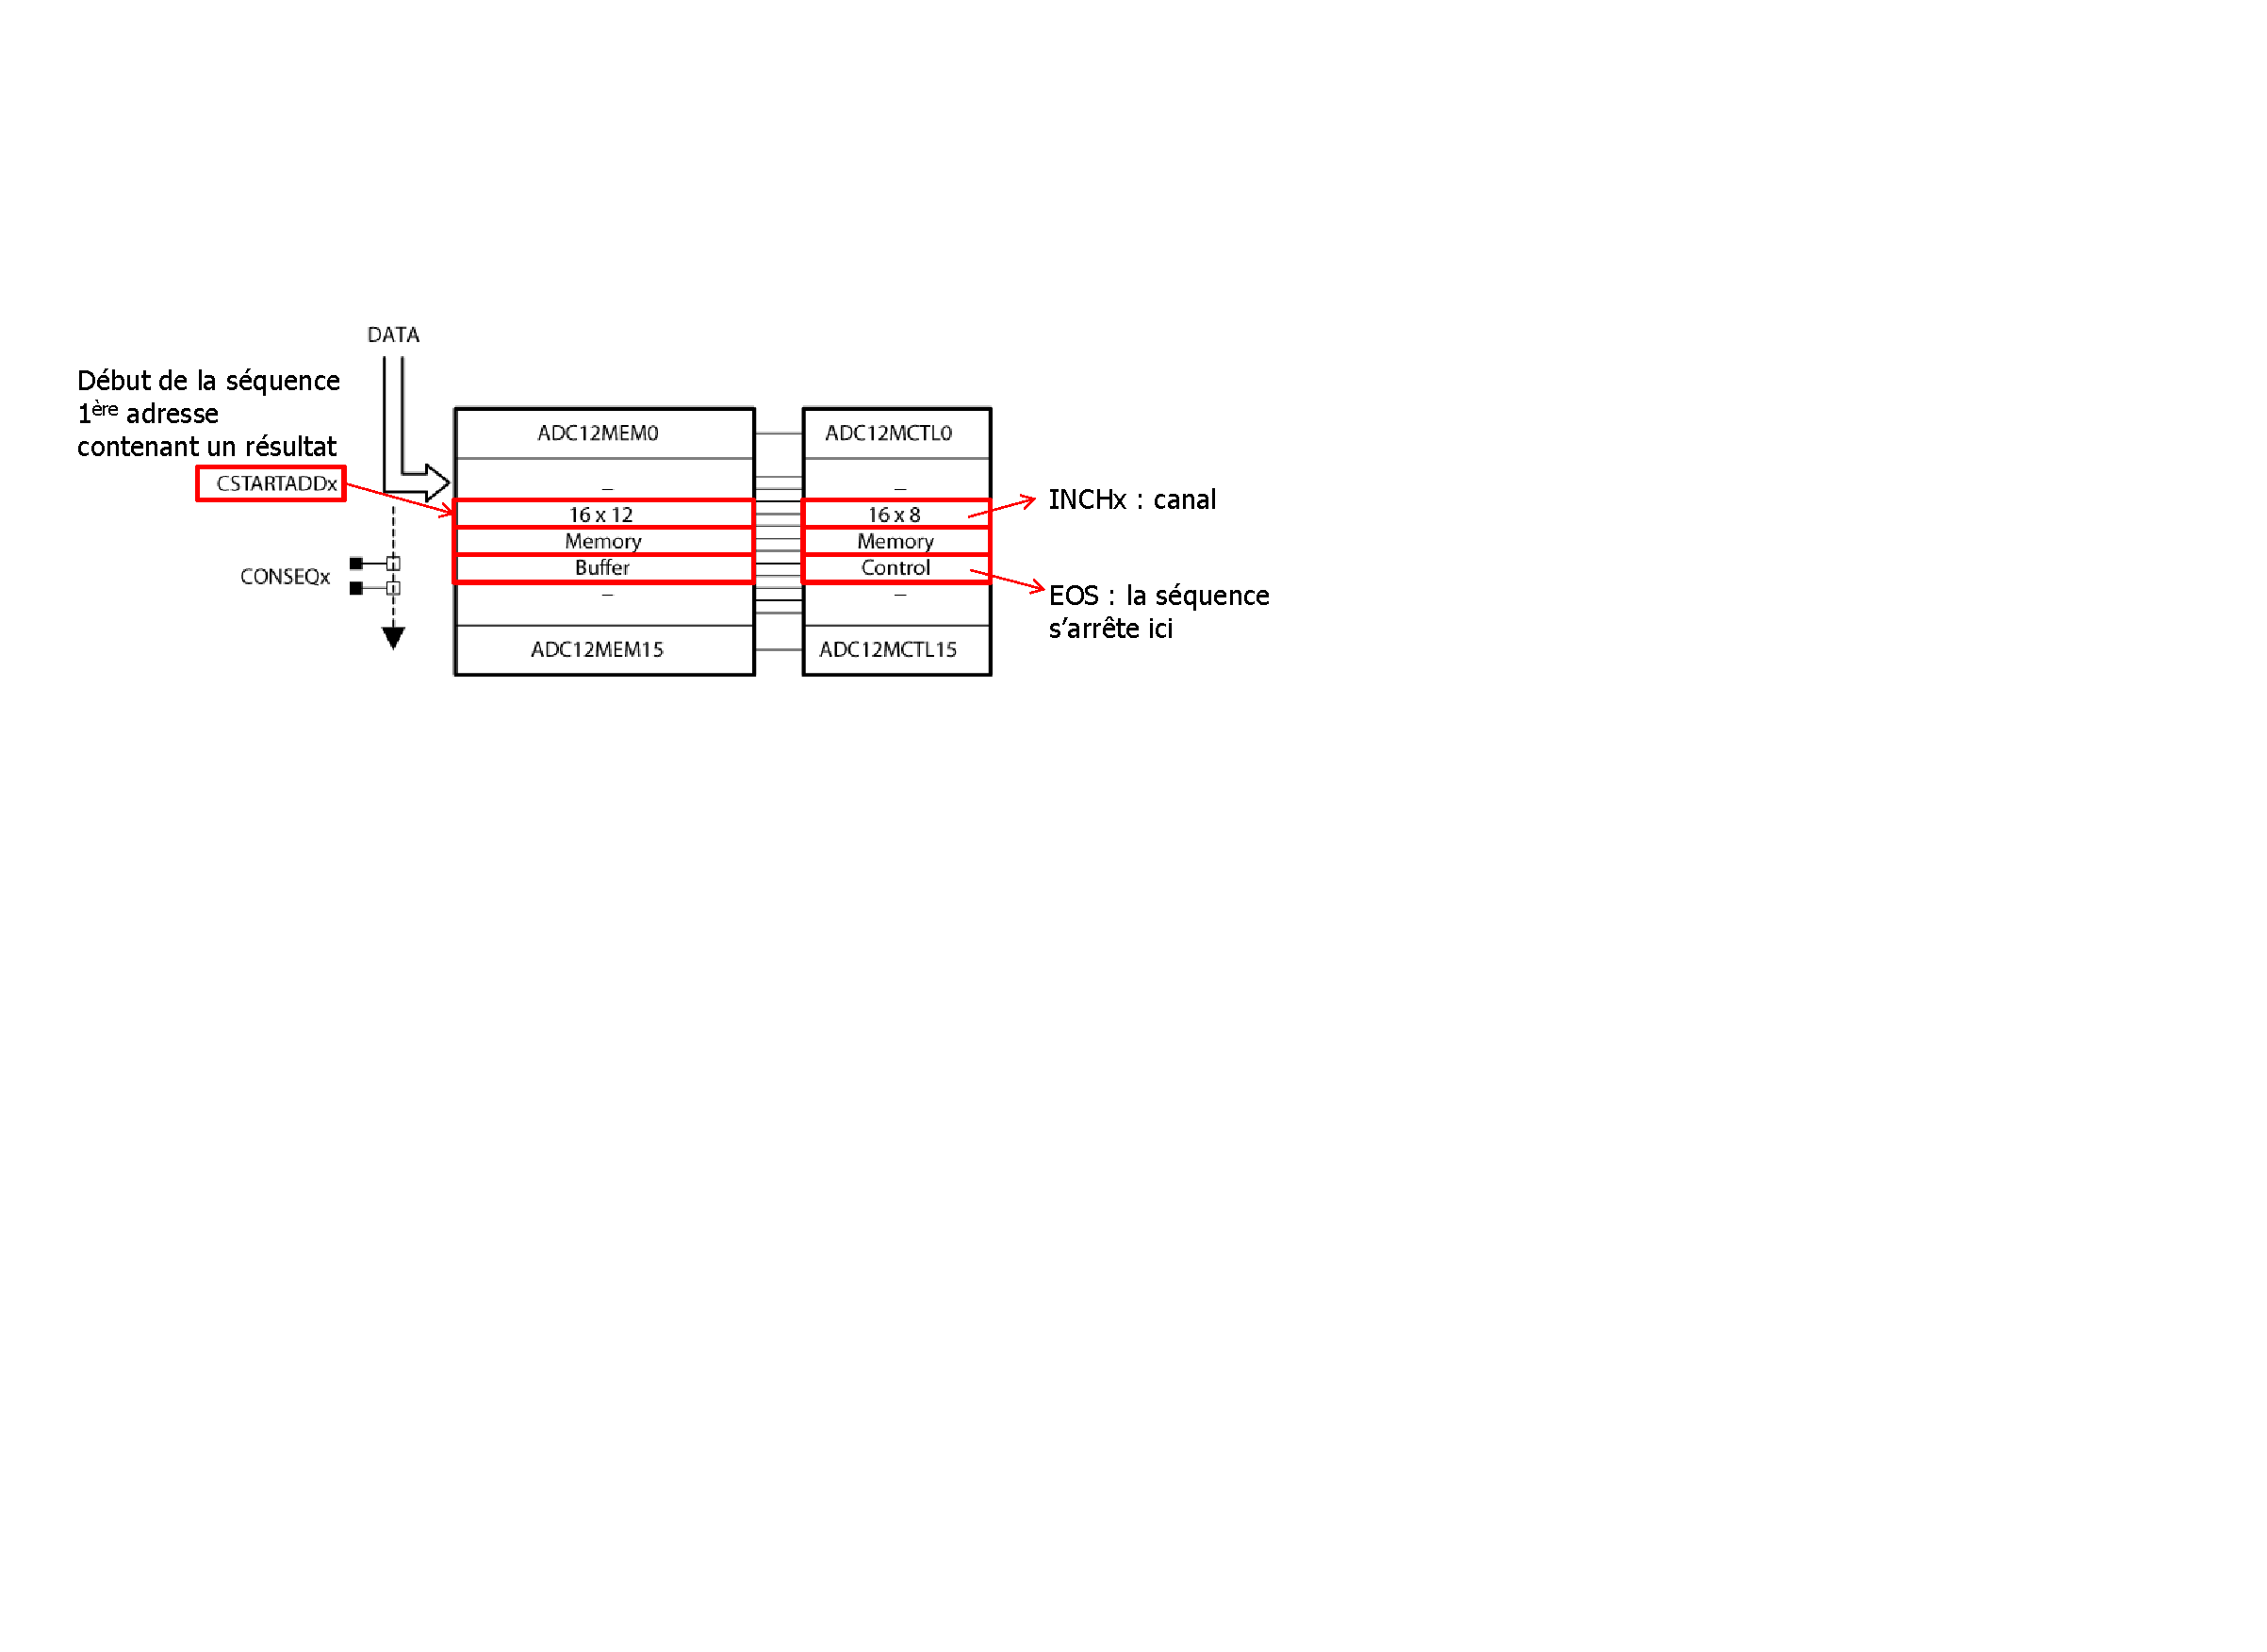
\includegraphics [angle=0, width=14cm]{./Figures/Chap11_ADC/ADC12Stockage.pdf}
  \rule{35em}{0.5pt}
  \caption{Organisation des registres de stockage et leur contrôle}
  \label{fig:ADC12Stockage}
\end{figure}

Un champ noté ADC12CSTARTADDx contient l'adresse du registre dans lequel se trouvera le résultat de la conversion. SI plusieurs conversions doivent être enchaînées, ce champ indique dans quel registre se trouve le premier résultat, les autres se trouvant dans les registres ADC12MEMx suivants.
Pour contrôler les conversions, chaque registre ADC12MCTLx contient 3 champs :
\begin{itemize}[label=\textbullet,font=\small]
\item INCHx : le numéro de l'entrée à convertir;
\item SREFx : le jeu de tensions de référence à utiliser;
\item EOS : le registre ADC12MCTLy contenant ce bit à '1' marque la fin de la séquence.
\end{itemize}

Ainsi, chaque conversion d'une séquence dispose de ses paramètres propres. Il est bien entendu possible de convertir le signal d'une seule entrée, auquel cas il s'agit d'une séquence d'une seule conversion.\\

Lors de l'écriture d'un résultat de conversion dans un registre, une requête d'interruption est émise. Dans le cas d'une séquence de conversions, il suffit de n'autoriser que celle correspondant à la fin de la séquence.

\pagebreak
\subsection{Registres de contrôle du convertisseur ADC12}

Ils sont nommés ADC12CTLx et sont au nombre de 3. Dans les tableaux suivants, on donne uniquement la signification des champs de contrôle les plus importants.

\begin{figure}[H]
  \centering
  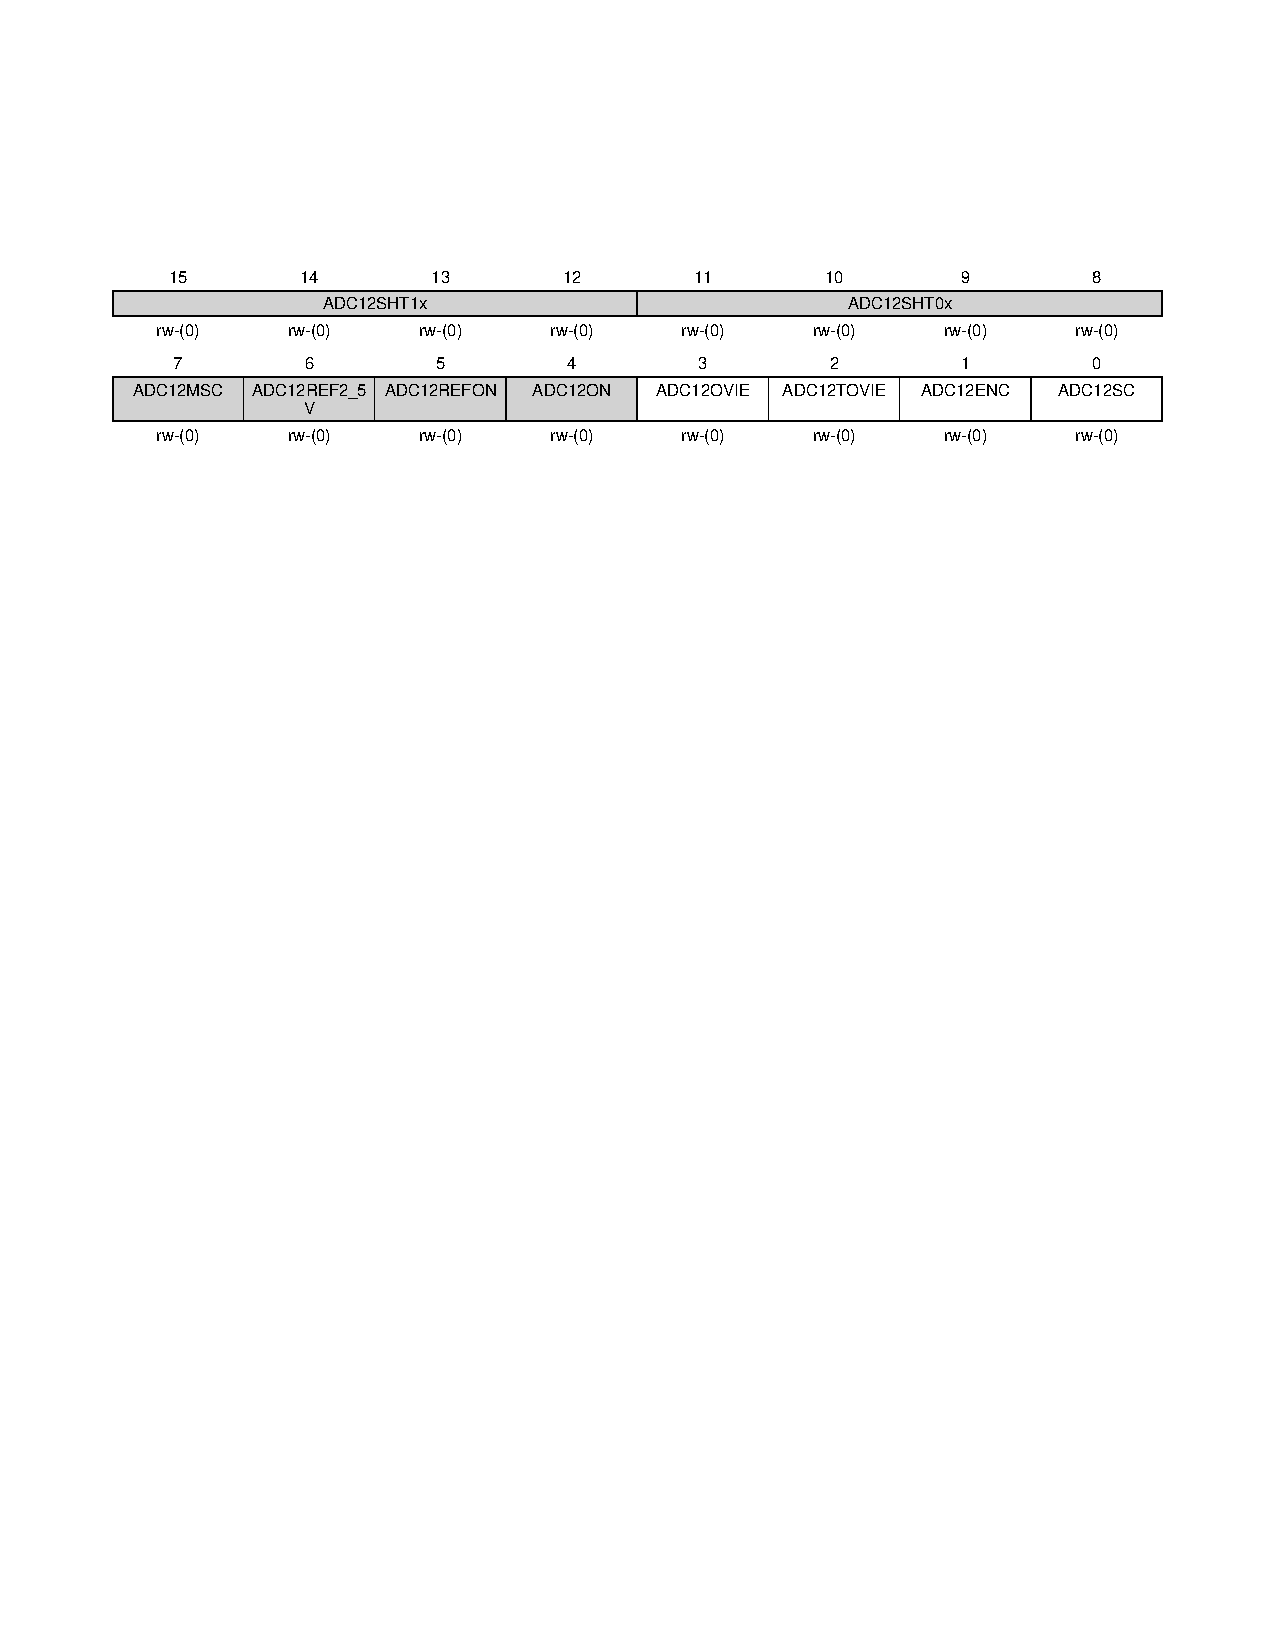
\includegraphics [angle=0, width=16cm]{./Figures/Chap11_ADC/ADC12CTL0.pdf}
  \rule{35em}{0.5pt}
  \caption{ADC12CTL0}
  \label{fig:ADC12CTL0}
\end{figure}

\begin{table}[H]
\centering 
\begin{tabular}{l l l l}
\hline\hline
Champ & & Valeur & Description \\ %[0.5ex]
\hline
ADC12SHT1 & & & Durée d'échantillonnage pour les conversions \\
& & & contrôlées par ADC12MCTL8 à ADC12MCTL15   \\
\hline
ADC12SHT0 & & & Durée d'échantillonnage pour les conversions \\
& & &  contrôlées par ADC12MCTL0 à ADC12MCTL7   \\
& & 0000b & 4 cycles de ADC12CLK \\
& & 0001b & 8 cycles de ADC12CLK \\
& & 0010b & 16 cycles de ADC12CLK \\
& & 0011b & 32 cycles de ADC12CLK \\
& & 0100b & 64 cycles de ADC12CLK \\
& & 0101b & 96 cycles de ADC12CLK \\
& & 0110b & 128 cycles de ADC12CLK \\
& & 0111b & 192 cycles de ADC12CLK \\
& & 1000b & 256 cycles de ADC12CLK \\
& & 1001b & 384 cycles de ADC12CLK \\
& & 1010b & 512 cycles de ADC12CLK \\
& & 1011b & 768 cycles de ADC12CLK \\
& & 11xxb & 1024 cycles de ADC12CLK \\
\hline
ADC12MSC & & - & Permet d'enchaîner des conversions multiples \\
\hline
ADC12ON & & - & Mise en marche du convertisseur \\
& & 0 & Convertisseur arrêté \\
& & 1 & Convertisseur en marche \\
\hline
ADC12ENC & & - & Lancement du contrôleur de conversions \\
& & 0 & Contrôleur arrêté \\
& & 1 & Contrôleur prêt \\
\hline
ADC12SC & & - & Lancement d'une conversion \\
& & 1 & Start \\
\hline
\end{tabular}
\caption{ADC12CTL0}
\label{table:ADC12CTL0}
\end{table}

\pagebreak
\begin{figure}[H]
  \centering
  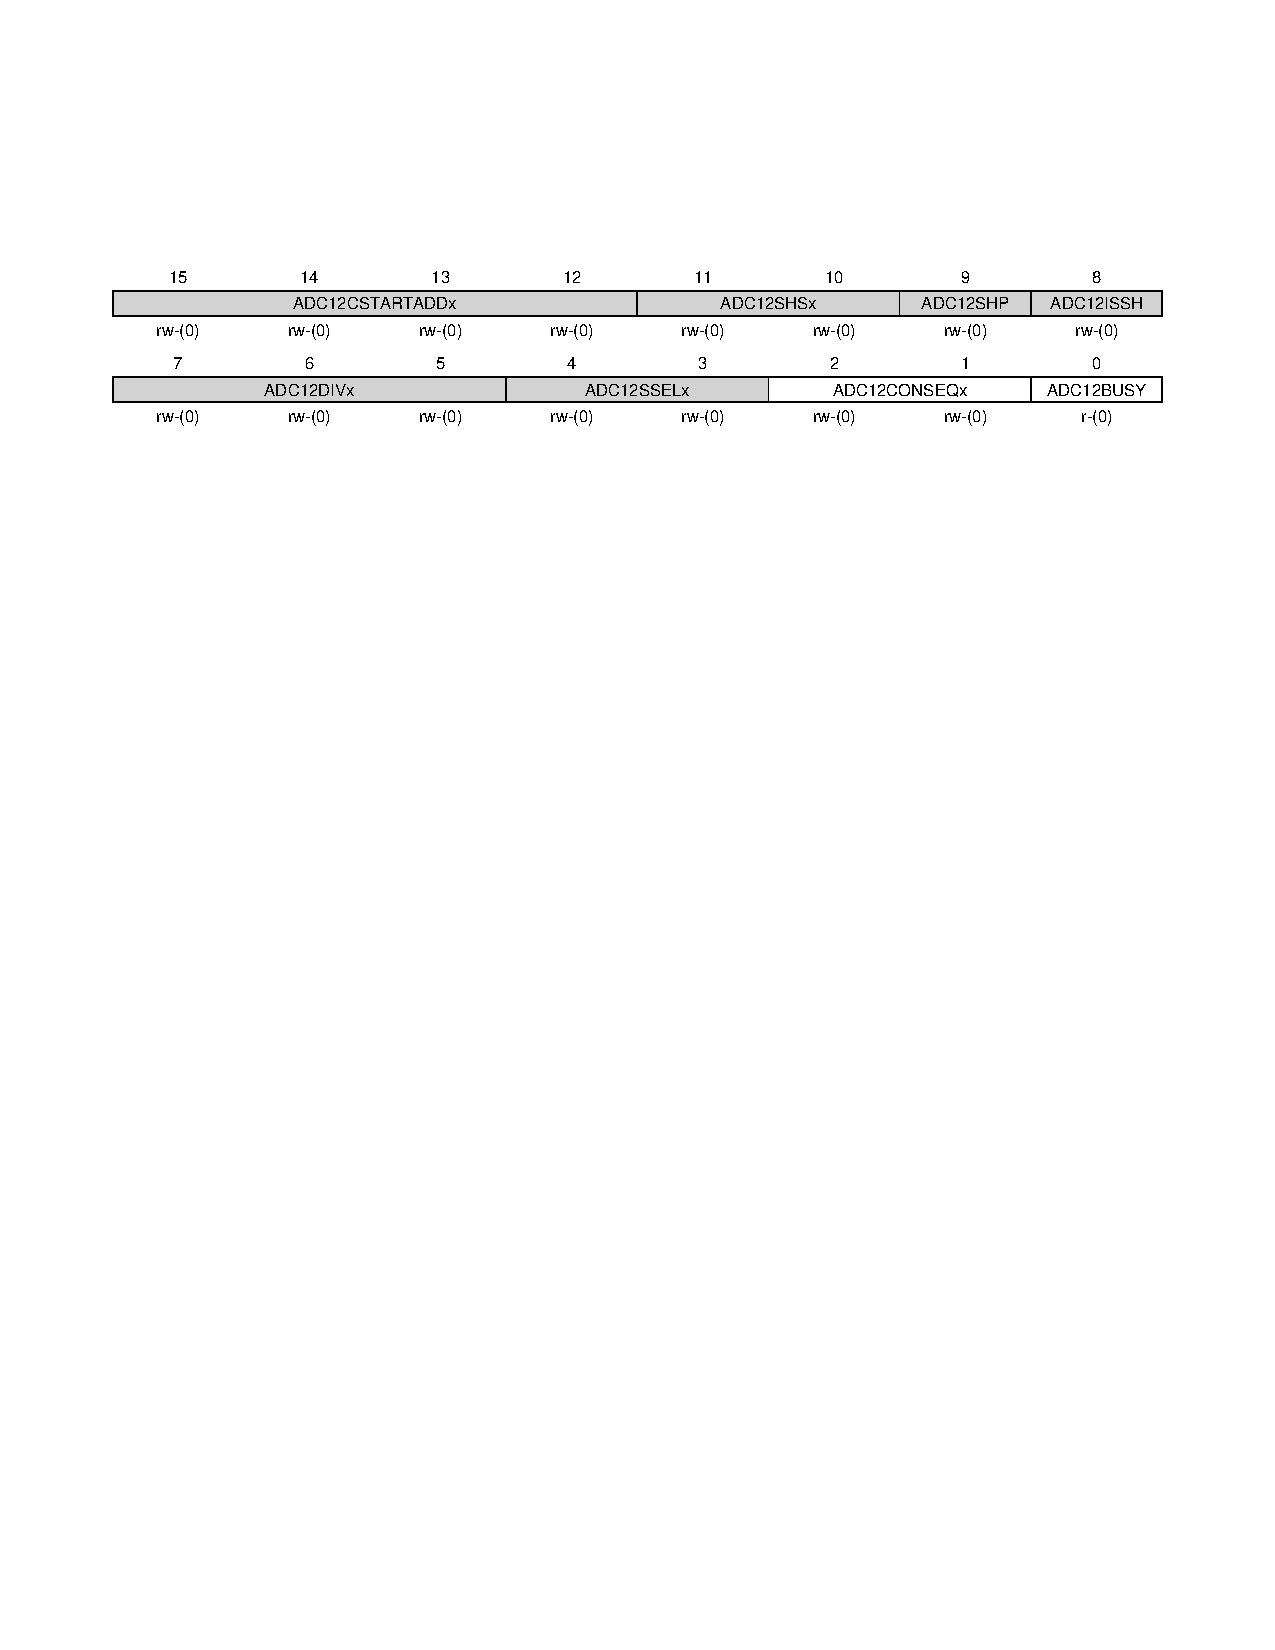
\includegraphics [angle=0, width=16cm]{./Figures/Chap11_ADC/ADC12CTL1.pdf}
  \rule{35em}{0.5pt}
  \caption{ADC12CTL1}
  \label{fig:ADC12CTL1}
\end{figure}

\begin{table}[H]
\centering 
\begin{tabular}{l l l l}
\hline\hline
Champ & & Valeur & Description \\ %[0.5ex]
\hline
ADC12CSTARTADD & & - & Adresse du registre de contrôle de la conversion \\
& & & ou de la première conversion, dans le cas d'une séquence \\
\hline
ADC12SHS & & & Sélection du signal de conversion \\
& & 00b & bit ADC12SC (lancement par logiciel) \\
& & 01b & timer (consulter la fiche technique du MCU) \\
& & 10b & timer (consulter la fiche technique du MCU) \\
& & 11b & timer (consulter la fiche technique du MCU) \\
\hline
ADC12SHP & & & Contrôle de la durée d'échantillonnage \\
& & 0 & SAMPCON égale le signal de conversion \\
& & 1 & Le niveau haut de SAMPCON est fixé par le timer de conversion \\
& & & voir le champ ADC12SHT0 ou ADC12SHT1 dans ADC12CTL0 \\
\hline
ADC12ISSH & & - & Inversion du signal de conversion (\ref{fig:ADC_Schema})\\
& & 0 & Pas d'inversion \\
& & 1 & Inversion \\
\hline
ADC12DIV & & - & Prédivision de l'horloge de conversion ADC12CLK \\
& & 000b & Division par 1 \\
& & 001b & Division par 2 \\
& & 010b & Division par 3 \\
& & ... & ... \\
& & 110b & Division par 7 \\
& & 111b & Division par 8 \\
\hline
ADC12SSEL & & - & Sélection de l'horloge de conversion ADC12CLK \\
& & 00b & ADC12OSC \\
& & 01b & ACLK \\
& & 10b & MCLK \\
& & 11b & SMCLK \\
\hline
ADC12CONSEQ & & - & Mode de conversion \\
& & 00b & Conversion unique sur un canal unique \\
& & 01b & Séquence de conversions \\
& & 10b & Canal unique en répétition \\
& & 11b & Séquence en répétition \\
\hline
ADC12BUSY & & - & Indicateur de conversion en cours\\
& & 0 & Pas de conversion en cours \\
& & 1 & Une conversion en cours \\
\hline
\end{tabular}
\caption{ADC12CTL1}
\label{table:ADC12CTL1}
\end{table}

\pagebreak
\begin{figure}[H]
  \centering
  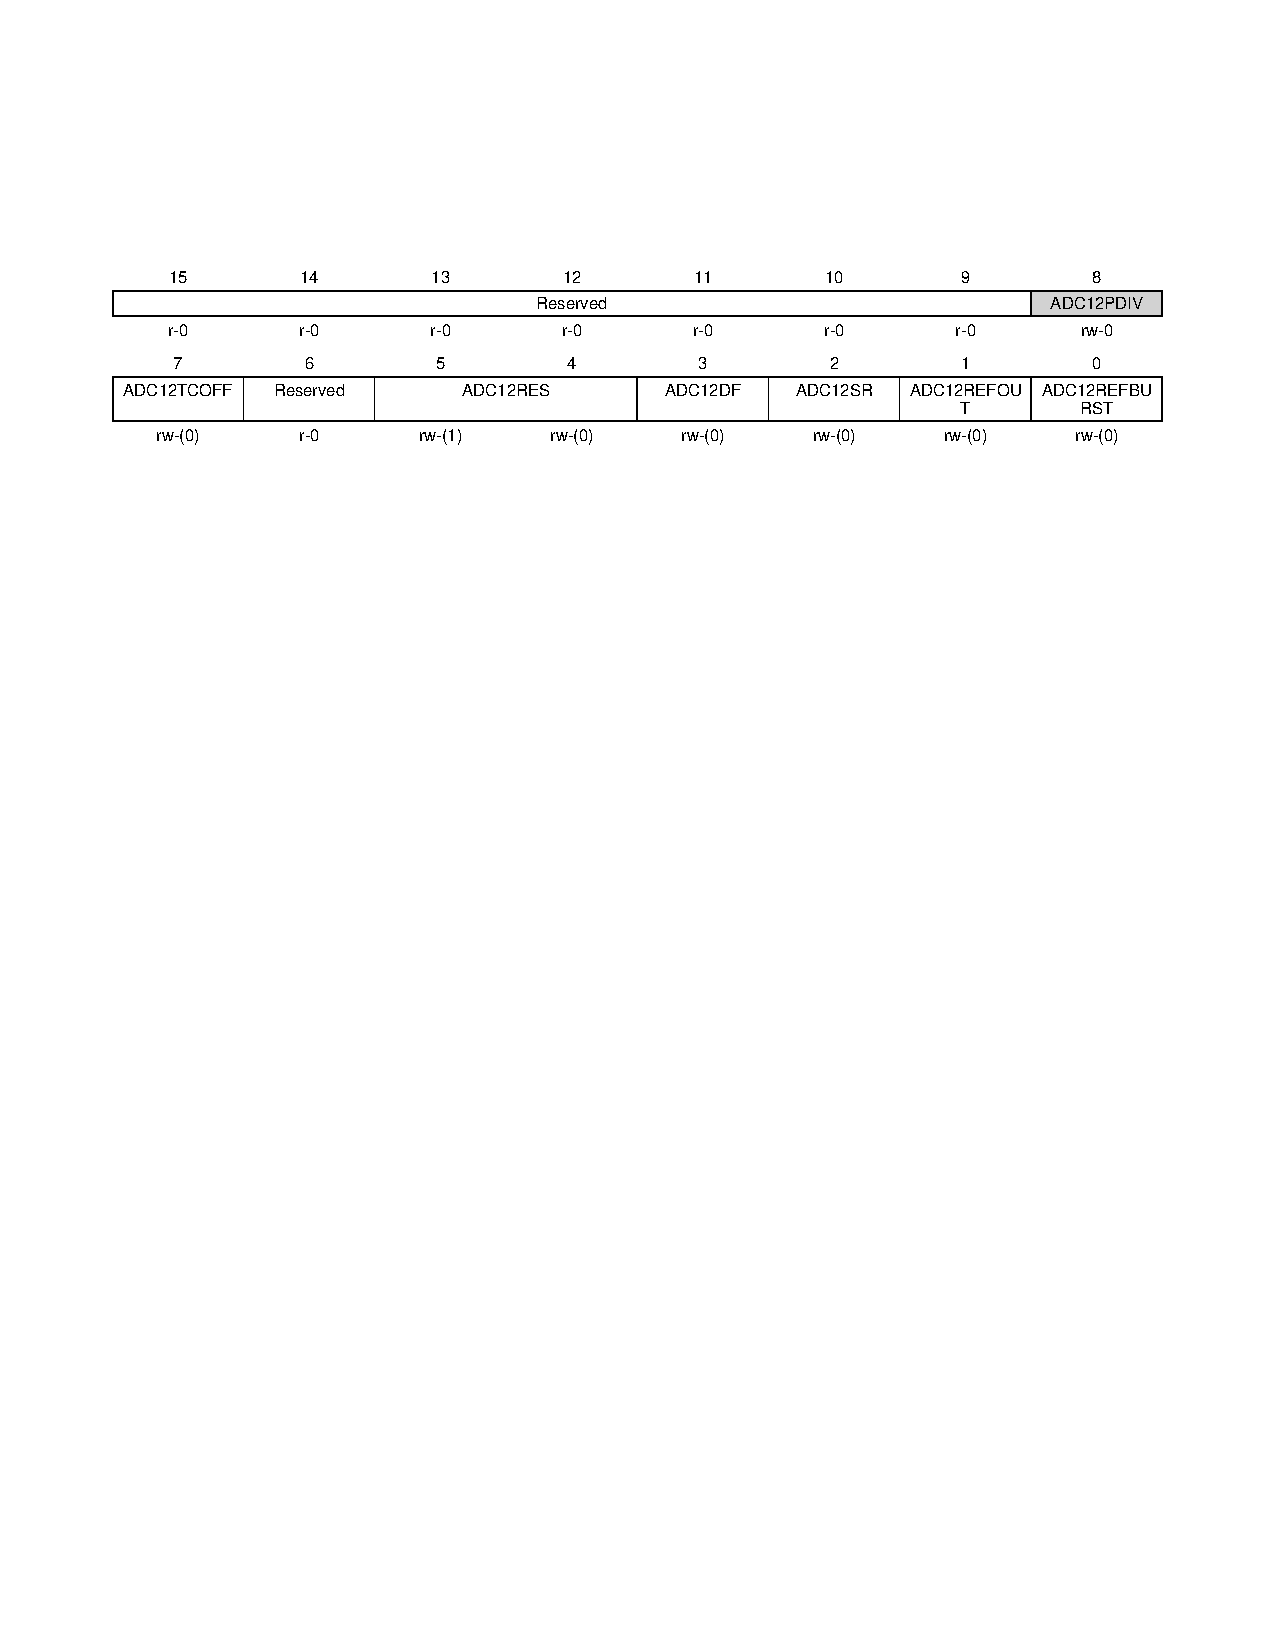
\includegraphics [angle=0, width=16cm]{./Figures/Chap11_ADC/ADC12CTL2.pdf}
  \rule{35em}{0.5pt}
  \caption{ADC12CTL2}
  \label{fig:ADC12CTL2}
\end{figure}

\begin{table}[H]
\centering 
\begin{tabular}{l l l l}
\hline\hline
Champ & & Valeur & Description \\ %[0.5ex]
\hline
ADC12PDIV & & - & Prédivision de l'horloge de conversion ADC12CLK \\
& & & en plus de la prédivision contrôlée par ADC12DIV \\
& & 0 & Prédivision par 1 \\
& & 1 & Prédivision par 4 \\
\hline
ADC12RES & & & Spécifie le nombre de bits du résultat de conversion \\
& & 00b & 8 bits (9 cycles de ADC12CLK) \\
& & 01b & 10 bits (11 cycles de ADC12CLK) \\
& & 10b & 12 bits (13 cycles de ADC12CLK) \\
& & 11b & Réservé \\
\hline
ADC12DF & & & Format du résultat de conversion sur 16-bits \\
& & 0 & Binaire non signé. -VREF = 0000h, +VREF = 0FFFh \\
& & & Le résultat est justifié à droite (vers les poids faibles) \\
& & 1 & Binaire signé. -VREF = 8000h, +VREF = 7FF0h \\
& & & Le résultat est justifié à gauche (vers les poids forts) \\
\hline
\end{tabular}
\caption{ADC12CTL2}
\label{table:ADC12CTL2}
\end{table}

\subsection{Exemples de configuration}

\begin{minipage}{16cm}{
\subsubsection*{Exemple 1}
L'entrée A0 est convertie sur ordre logiciel. La référence est AVcc. ADC12SC est remis à 0 automatiquement à la fin de la conversion. Le résultat est dans ADC12MEM0. Dans la boucle principale, le CPU attend en LPM0 jusqu'à l'interruption de ADC12. Au retour de l'interruption, le CPU ne retourne pas en LPM0 pour pouvoir lancer une nouvelle conversion. Si A0 > 0.5*AVcc, P1.0 est mis à '1', sinon '0'.

\lstset{style=customc}
\begin{lstlisting}
//*******************************************************************
// MSP430F552x Demo - MSP430F55xx_adc_01
// Bhargavi Nisarga, Texas Instruments Inc.
//*******************************************************************
#include <msp430.h>

void main(void)
{
  WDTCTL = WDTPW + WDTHOLD;              // Stop le watchdog timer

  ADC12CTL0 = ADC12SHT02 + ADC12ON;      // Temps d'échant., ADC12 on
  ADC12CTL1 = ADC12SHP;                  // Timer d'échant. (SHP = 1)
  ADC12IE = 0x01;                        // Interruption autorisée
  ADC12CTL0 |= ADC12ENC;                 // Armement de l'ADC
  P6SEL |= 0x01;                         // P6.0 mis en connection avec A0
  P1DIR |= 0x01;                         // P1.0 en sortie

  while (1)
  {
    ADC12CTL0 |= ADC12SC;                // Lancer échant./conversion
    __bis_SR_register(LPM0_bits + GIE);  // LPM0
  }
}

#pragma vector = ADC12_VECTOR
__interrupt void adc12_isr(void)
{
  switch(__even_in_range(ADC12IV,34))
  {
  case  0: break;                        // Vecteur  0:  Pas d'interruption
  case  2: break;                        // Vecteur  2:  ADC overflow
  case  4: break;                        // Vecteur  4:  ADC timing overflow
  case  6:                               // Vecteur  6:  ADC12IFG0
    if (ADC12MEM0 >= 0x7ff)              // ADC12MEM = A0 > 0.5*AVcc?
      P1OUT |= BIT0;                     // P1.0 = 1
    else
      P1OUT &= ~BIT0;                    // P1.0 = 0
    __bic_SR_register_on_exit(LPM0_bits);// le CPU ne retournera pas en LPM0
    break;
  case  8: break;                        // Vecteur  8:  ADC12IFG1
  case 10: break;                        // Vecteur  10: ADC12IFG2
  case 12: break;                        // Vecteur  12: ADC12IFG3
  case 14: break;                        // Vecteur  14: ADC12IFG4
  ...
  case 16 à 28 omis pour des raisons de mise en page
  ...
  case 30: break;                        // Vecteur  30: ADC12IFG12
  case 32: break;                        // Vecteur  32: ADC12IFG13
  case 34: break;                        // Vecteur  34: ADC12IFG14
  default: break; 
  }
}
\end{lstlisting}
}
\end{minipage}

\begin{minipage}{16cm}{
\subsubsection*{Exemple 2}
Les entrées A0 à A3 sont converties en séquence. Les références sont AVcc.
Les résultats sont dans ADC12MEM0-3. Dans la boucle principale, le CPU attend en LPM4 jusqu'à l'interruption.

\lstset{style=customc}
\begin{lstlisting}
//*******************************************************************
// MSP430F552x Demo - MSP430F55xx_adc_09
// Bhargavi Nisarga, Texas Instruments Inc.
//*******************************************************************

#include <msp430.h>
#include <stdint.h>

volatile uint16_t results[4];          // tableau pour stocker les résultats

void main(void)
{
  WDTCTL = WDTPW+WDTHOLD;                  // Stop watchdog timer

  P6SEL = 0x0F;                            // P6.0-3 connectés avec A0-A3

  ADC12CTL0 = ADC12ON+ADC12MSC+ADC12SHT0_2;// Temps d'échant., ADC12 on
  ADC12CTL1 = ADC12SHP + ADC12CONSEQ_1;    // Timer d'échant., séq. simple
  ADC12MCTL0 = ADC12INCH_0;                // ref+ = AVcc, channel = A0
  ADC12MCTL1 = ADC12INCH_1;                // idem channel A1
  ADC12MCTL2 = ADC12INCH_2;                // idem channel A2
  ADC12MCTL3 = ADC12INCH_3+ADC12EOS;       // idem channel A3, fin séquence
  ADC12IE = 0x08;                          // Autorisation ADC12IFG.3
  ADC12CTL0 |= ADC12ENC;                   // Armement de l'ADC

  while(1)
  {
    ADC12CTL0 |= ADC12SC;                  // Lancer échant./conversion
    __bis_SR_register(LPM4_bits + GIE);    // LPM4, autorisation interrupts
  }
}

#pragma vector=ADC12_VECTOR
__interrupt void adc12_isr(void)
{
  switch(__even_in_range(ADC12IV,34))
  {
  case  0: break;                        // Vecteur  0:  No interrupt
  case  2: break;                        // Vecteur  2:  ADC overflow
  case  4: break;                        // Vecteur  4:  ADC timing overflow
  case  6: break;                        // Vecteur  6:  ADC12IFG0
  case  8: break;                        // Vecteur  8:  ADC12IFG1
  case 10: break;                        // Vecteur  10:  ADC12IFG2
  case 12:                               // Vecteur  12:  ADC12IFG3
    results[0] = ADC12MEM0;              // sauver résultat, IFG remis à 0
    results[1] = ADC12MEM1;              // sauver résultat, IFG remis à 0
    results[2] = ADC12MEM2;              // sauver résultat, IFG remis à 0
    results[3] = ADC12MEM3;              // sauver résultat, IFG remis à 0
    __bic_SR_register_on_exit(LPM4_bits);// le CPU ne retournera pas en LPM4
    break;
  case 14: break;                        // Vecteur  14:  ADC12IFG4
  // case 16 à 32 omis pour des raisons de mise en page
  case 34: break;                           // Vector 34:  ADC12IFG14
  default: break; 
  }
}
\end{lstlisting}
}
\end{minipage}
